\documentclass[a4paper]{article}

\usepackage[portuguese]{babel}
\usepackage[utf8]{inputenc}
\usepackage{graphicx,hyperref}
\usepackage{float}
\usepackage{listings}
\usepackage{proof,tikz}
\usepackage{algorithm2e}
\usepackage{amssymb,amsthm,stmaryrd}


\usepackage[edges]{forest}
\usetikzlibrary{automata, positioning, arrows}


\newtheorem{Lemma}{Lema}
\newtheorem{Theorem}{Teorema}
\theoremstyle{definition}
\newtheorem{Example}{Exemplo}
\newtheorem{Definition}{Definição}
\newtheorem{Fact}{Fato}


\usepackage{fancyhdr}
  \pagestyle{fancy}
  \fancyhf{}
  \lhead{Teoria da Computação}
  \rhead{Aula 24}
  \lfoot{Prof. Rodrigo Ribeiro}
  \rfoot{\thepage}
  \renewcommand{\footrulewidth}{0.4pt}
  \pagestyle{fancy}

\tikzset{
        ->,  % makes the edges directed
        >=stealth', % makes the arrow heads bold
        node distance=3cm,
        every state/.style={thick, fill=gray!10},
        initial text=$\,$
        }
  

\begin{document}

\title{Aula 24 - Redução de Problemas}
  \author{Rodrigo Ribeiro}

  \maketitle

  \pagestyle{fancy}


  \section*{Objetivos}

  \begin{itemize}
     \item Apresentar o conceito de redução de problemas e mostrar como
           esse pode ser utilizado para demonstrar a decidibilidade de problemas.
  \end{itemize}


  \section{Introdução}

  Existem duas técnicas principais para demonstração de indecidibilidade de
  problemas: \emph{diagonalização} e \emph{redução}. A diagonalização consiste
  em uma argumentação similar à feita  na demonstração do teorema de Cantor e
  é exatamente o estilo de prova utilizado para mostrar a indecidibilidade do
  problema da parada.

  Outra forma para demonstrar a indecidibilidade de problema é por redução.
  Na aula 23, mostrarmos que o problema da parada é indecidível. Podemos mostrar
  que um problema $P$ é indecidível reduzindo o problema da parada a $P$.
  Intuitivamente, isso significa que podemos manipular entradas para o problema
  da parada para torná-las ``similares'' às entradas de $P$ de forma que
  possamos usar $P$ para resolver o problema da parada. Porém, como sabemos que
  o problema da parada é indecidível, podemos concluir por contradição que $P$
  também o deve ser.

  \section{Redução}

  \begin{Definition}
    Sejam $A \subseteq \Sigma^*$ e $B \subseteq \Delta^*$ duas linguagens sobre
    alfabetos $\Sigma$ e $\Delta$. Uma redução de $A$ para $B$ é uma função
    computável (MT):
    \[
      \sigma : \Sigma^*\to \Delta^*
    \]
    tal que para todo $x \in \Sigma^*$, $x \in A \leftrightarrow\sigma(x) \in B $.
  \end{Definition}

  De maneira intuitiva, a condição
  \[
    x \in A \leftrightarrow\sigma(x) \in B 
  \]
  expressa que palavras em $A$ devem ser associadas a palavras em $B$ pela
  função $\sigma$, e palavras que não estão em $A$ devem ser associadas a
  palavras que não estão em $B$ sobre $\sigma$. A figura seguinte ilustra essa
  situação.
  \begin{figure}[H]
    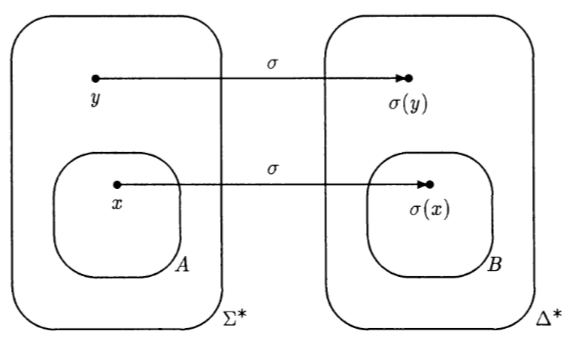
\includegraphics[scale=.4]{reduction.png}
    \centering
  \end{figure}
  É importante salientar que não há necessidade de $\sigma$ ser uma função
  bijetora. A única exigência sobre $\sigma$ é que esta seja uma função total e
  computável (i.e. existe uma MT que a calcule e pare para todas as palavras).

  Porém, pode restar a pergunta: como definir uma MT que calcula uma função?
  A idéia é que a MT receba uma palavra $w \in A$ e pare com a fita contendo
  a palavra $\sigma(w) \in B$. Expressamos que $A$ é redutível a $B$ por uma
  função $\sigma$ como $A\leq_\sigma B$. É fácil ver que a relação $\leq_\sigma$
  é reflexiva e transitiva.

  \section{Provas por redução}
  
  Conforme discutido anteriormente, provar a indecidibilidade de um problema
  por redução consiste em ``transformar'' entradas de um problema sabidamente
  indecidível para entradas do problema cuja indecibilidade desejamos provar ($P$) de
  forma que seja possível obter a resposta do problema indecidível usando $P$.
  Porém, como mostrar a decidibilidade de problemas? Podemos usar redução para
  esse fim. Para isso, basta reduzir $P$ a um problema que sabemos ser
  decidível.

  Resumindo:

  \begin{itemize}
     \item Para demonstrar que um problema $P$ é indecidível, basta reduzir um
       problema indecidível a $P$;
     \item Para demonstrar que um problema $P$ é decidível, basta reduzir $P$ a
       um problema decidível.
  \end{itemize}

  \begin{Example}
    Vamos mostrar que o problema de ``determinar se $L(M)$ é finita, em que $M$
    é um AFD'' é decidível. Para isso, vamos reduzir o problema $L(M)$ é finita
    ao problema decidível de determinar se um grafo possui ciclos. Observe que a
    entrada para uma MT que resolve a questão $L(M)$ é finita é $R\langle M
    \rangle$, que consiste de uma representação de um AFD como uma palavra sobre
    um alfabeto $\Sigma$. A função de redução será uma MT que converte a
    representação de AFD para uma representação de grafos.

    Como sabemos que $L(M)$ é infinita se o grafo de seu AFD possui ciclos, e
    pode-se converter entre representações de AFD em uma representação de grafo,
    temos que o problema em questão é decidível, visto que determinar se um
    grafo possui ciclos também o é.
  \end{Example}

  O próximo exemplo mostra o uso de redução para demonstrar a indecidibilidade
  de um problema.

  \begin{Example}
    O problema da fita em branco pode ser enunciado da seguinte forma: dada uma
    MT $M$, determinar se $M$ para com entrada $\lambda$. Mostraremos que o
    problema da fita em branco é indecidível reduzindo-o ao problema da parada.
    Para isso, vamos definir uma função $\sigma$ que a partir de uma entrada
    $R\langle M,w \rangle$ para o problema da parada produz uma palavra
    $R\langle M' \rangle$ que denota o problema da fita em branco de forma que
    $M'$ pare com entrada $\lambda$ se, e somente se, $M$ para com entrada $w$.

    Porém, como especificar a função $\sigma$? A idéia é especificar a
    transformação que $\sigma$ realiza sobre a entrada em ``alto-nível''.
    Apesar de usarmos uma descrição de alto-nível, os passos realizados devem
    concluir em tempo finito, garantindo a computabilidade de $\sigma$.
    Para o caso do problema da fita em branco, a função $\sigma$ deve produzir
    $R\langle M' \rangle$ a partir de $R\langle M,w \rangle$ de forma que
    $M'$ possua o seguinte comportamento:
    \begin{enumerate}
      \item $M'$ apaga a entrada. Esse passo é simples, basta adicionar um novo
        estados $l_1,l_2$ a $M$ com transições que apagam o conteúdo da fita até
        alcançar a primeiro símbolo de $\sqcup$. As transições incluídas seriam:
        \begin{itemize}
          \item $\delta(l_1,a) = [l_1,\sqcup,D]$, para todo $a \in \Gamma
            -\{\langle\}$
          \item $\delta(l_1,\sqcup) = [l_2,\sqcup,E]$
          \item $\delta(l_2, \sqcup) = [l_2,\sqcup,E]$
          \item $\delta(l_2,\langle) = [i,\langle, D]$, em que $i$ é o estado
            inicial de $M$
          \end{itemize}
       \item $M'$ escreve $w$. Se $|w| = n$, então basta incluir $n + 2$ estados
         a MT resultante do passo anterior contendo transições para escrever cada
         um dos símbolos de $w$, que demanda $n + 1$ estados, e um último estado
         para voltar a fita ao início.
       \item A partir desse passo, $M'$ comporta-se exatamente como $M$. Isto é,
         o restando dos estados e transições de $M'$ são exatamente os originais
         de $M$.
    \end{enumerate}
    Com isso, temos que a $MT$ $M'$ pára com a fita em branco se, e somente se,
    a MT $M$ para com a entrada $w$. Dessa forma, temos que o problema da fita
    em branco é indecidível. 
  \end{Example}

  Dizer que um problema é indecidível resume-se a mostrar que a linguagem
  de códigos de MTs que o solucionam não é uma linguagem recursiva. No caso do
  problema da fita em branco, a sua prova de indecidibilidade representa o fato
  de que a linguagem
  \[
    \{R\langle M \rangle\,|\,\lambda\in L(M)\}
  \]
  não é recursiva.

  A seguir mostramos outro exemplo de prova de indecidibilidade.

  \begin{Example}
    Considere o seguinte problema: ``determinar se a linguagem de uma MT $M$ não
    é $\emptyset$''. Vamos mostrar que esse problema é indecidível reduzindo o
    problema da parada a este. Para isso, vamos definir uma MT $\sigma$ que
    transforma a entrada do problema da parada, $R\langle M,w \rangle$, na
    entrada do referido problema, $R\langle M' \rangle$. A função $\sigma$
    construirá $R\langle M' \rangle$ de forma que a MT $M'$ se comporte da
    seguinte maneira:
    \begin{enumerate}
      \item $M'$ apaga a palavra de entrada. Esse passo pode ser realizado
        conforme descrito na demonstração de indecidibilidade do problema da
        fita em branco.
      \item $M'$ escreve $w$ e volta o cabeçote ao início da fita.
      \item $M'$ se comporta como $M$.
    \end{enumerate}
    Dessa forma, temos que $M'$ para com alguma palavra (e portanto $L(M') \neq
    \emptyset$) se, e somente se, $M$ para com entrada $w$.
  \end{Example}
  
  \section{Exercícios}

  \begin{enumerate}
     \item Apresente uma codificação para AFDs e outra para grafos. Explique,
       usando um pseudo-código, como converter sua codificação de AFD para
       codificação de grafos.
     \item Para cada um dos problemas seguintes, mostre que esse é decidível ou
       não fornecendo uma prova por redução.
       \begin{enumerate}
          \item Dada uma MT $M$ e um número $n \in \mathbb{N}$, determinar se
            $M$ pára em $n$ passos.
          \item Dada uma MT $M$ e uma palavra $w$, determinar se $M$ move
            o cabeçote à esquerda durante o processamento de $w$.
          \item Dada uma MT $M$, uma palavra $w$ e um estado $e$, determinar
            se a computação de $w$ por $M$ atinge o estado $e$.
       \end{enumerate}
  \end{enumerate}
\end{document}
